% Options for packages loaded elsewhere
\PassOptionsToPackage{unicode}{hyperref}
\PassOptionsToPackage{hyphens}{url}
\PassOptionsToPackage{dvipsnames,svgnames,x11names}{xcolor}
%
\documentclass[
  12pt]{article}

\usepackage{amsmath,amssymb}
\usepackage{setspace}
\usepackage{iftex}
\ifPDFTeX
  \usepackage[T1]{fontenc}
  \usepackage[utf8]{inputenc}
  \usepackage{textcomp} % provide euro and other symbols
\else % if luatex or xetex
  \usepackage{unicode-math}
  \defaultfontfeatures{Scale=MatchLowercase}
  \defaultfontfeatures[\rmfamily]{Ligatures=TeX,Scale=1}
\fi
\usepackage{lmodern}
\ifPDFTeX\else  
    % xetex/luatex font selection
\fi
% Use upquote if available, for straight quotes in verbatim environments
\IfFileExists{upquote.sty}{\usepackage{upquote}}{}
\IfFileExists{microtype.sty}{% use microtype if available
  \usepackage[]{microtype}
  \UseMicrotypeSet[protrusion]{basicmath} % disable protrusion for tt fonts
}{}
\makeatletter
\@ifundefined{KOMAClassName}{% if non-KOMA class
  \IfFileExists{parskip.sty}{%
    \usepackage{parskip}
  }{% else
    \setlength{\parindent}{0pt}
    \setlength{\parskip}{6pt plus 2pt minus 1pt}}
}{% if KOMA class
  \KOMAoptions{parskip=half}}
\makeatother
\usepackage{xcolor}
\setlength{\emergencystretch}{3em} % prevent overfull lines
\setcounter{secnumdepth}{5}
% Make \paragraph and \subparagraph free-standing
\ifx\paragraph\undefined\else
  \let\oldparagraph\paragraph
  \renewcommand{\paragraph}[1]{\oldparagraph{#1}\mbox{}}
\fi
\ifx\subparagraph\undefined\else
  \let\oldsubparagraph\subparagraph
  \renewcommand{\subparagraph}[1]{\oldsubparagraph{#1}\mbox{}}
\fi


\providecommand{\tightlist}{%
  \setlength{\itemsep}{0pt}\setlength{\parskip}{0pt}}\usepackage{longtable,booktabs,array}
\usepackage{calc} % for calculating minipage widths
% Correct order of tables after \paragraph or \subparagraph
\usepackage{etoolbox}
\makeatletter
\patchcmd\longtable{\par}{\if@noskipsec\mbox{}\fi\par}{}{}
\makeatother
% Allow footnotes in longtable head/foot
\IfFileExists{footnotehyper.sty}{\usepackage{footnotehyper}}{\usepackage{footnote}}
\makesavenoteenv{longtable}
\usepackage{graphicx}
\makeatletter
\def\maxwidth{\ifdim\Gin@nat@width>\linewidth\linewidth\else\Gin@nat@width\fi}
\def\maxheight{\ifdim\Gin@nat@height>\textheight\textheight\else\Gin@nat@height\fi}
\makeatother
% Scale images if necessary, so that they will not overflow the page
% margins by default, and it is still possible to overwrite the defaults
% using explicit options in \includegraphics[width, height, ...]{}
\setkeys{Gin}{width=\maxwidth,height=\maxheight,keepaspectratio}
% Set default figure placement to htbp
\makeatletter
\def\fps@figure{htbp}
\makeatother

\addtolength{\oddsidemargin}{-.5in}%
\addtolength{\evensidemargin}{-1in}%
\addtolength{\textwidth}{1in}%
\addtolength{\textheight}{1.7in}%
\addtolength{\topmargin}{-1in}%
\makeatletter
\@ifpackageloaded{caption}{}{\usepackage{caption}}
\AtBeginDocument{%
\ifdefined\contentsname
  \renewcommand*\contentsname{Table of contents}
\else
  \newcommand\contentsname{Table of contents}
\fi
\ifdefined\listfigurename
  \renewcommand*\listfigurename{List of Figures}
\else
  \newcommand\listfigurename{List of Figures}
\fi
\ifdefined\listtablename
  \renewcommand*\listtablename{List of Tables}
\else
  \newcommand\listtablename{List of Tables}
\fi
\ifdefined\figurename
  \renewcommand*\figurename{Figure}
\else
  \newcommand\figurename{Figure}
\fi
\ifdefined\tablename
  \renewcommand*\tablename{Table}
\else
  \newcommand\tablename{Table}
\fi
}
\@ifpackageloaded{float}{}{\usepackage{float}}
\floatstyle{ruled}
\@ifundefined{c@chapter}{\newfloat{codelisting}{h}{lop}}{\newfloat{codelisting}{h}{lop}[chapter]}
\floatname{codelisting}{Listing}
\newcommand*\listoflistings{\listof{codelisting}{List of Listings}}
\makeatother
\makeatletter
\makeatother
\makeatletter
\@ifpackageloaded{caption}{}{\usepackage{caption}}
\@ifpackageloaded{subcaption}{}{\usepackage{subcaption}}
\makeatother
\ifLuaTeX
  \usepackage{selnolig}  % disable illegal ligatures
\fi
\usepackage[]{natbib}
\bibliographystyle{agsm}
\usepackage{bookmark}

\IfFileExists{xurl.sty}{\usepackage{xurl}}{} % add URL line breaks if available
\urlstyle{same} % disable monospaced font for URLs
\hypersetup{
  pdftitle={Assessing the Impact of Outliers on Least Square Variogram Model},
  pdfauthor={Caterina Daidone, Marco Zanotti},
  pdfkeywords={geostatistics, outliers, variogram, robust statistics},
  colorlinks=true,
  linkcolor={blue},
  filecolor={Maroon},
  citecolor={Blue},
  urlcolor={Blue},
  pdfcreator={LaTeX via pandoc}}


\begin{document}


\def\spacingset#1{\renewcommand{\baselinestretch}%
{#1}\small\normalsize} \spacingset{1}


%%%%%%%%%%%%%%%%%%%%%%%%%%%%%%%%%%%%%%%%%%%%%%%%%%%%%%%%%%%%%%%%%%%%%%%%%%%%%%

\date{February 28, 2024}
\title{\bf Assessing the Impact of Outliers on Least Square Variogram
Model}
\author{
Caterina Daidone, Marco Zanotti\\
University of Milano Bicocca\\
}
\maketitle

\bigskip
\bigskip
\begin{abstract}
It is a matter of common experience that ore values often do not follow
the normal (or lognormal) distributions assumed for them, but, instead,
follow some other heavier-tailed distribution. This study reviews the
two most popular methods for the variogram estimation, that is the
classical and the robust variograms. Moreover, a simulation study is
performed to assess the impact of outliers on the variogram estimates.
It is shown that the use of the robust variogram yields stable estimates
when the scale of the contamination increases.
\end{abstract}

\noindent%
{\it Keywords:} geostatistics, outliers, variogram, robust statistics
\vfill

\newpage
\spacingset{1.9} % DON'T change the spacing!

\setstretch{1.5}
\section{Introduction}\label{introduction}

Spatial data consist of observations measured at known specific
locations or within specific regions and show regularities in space.
Remembering that the first law of geography states that ``everything is
related to everything else, but near things are more related than
distant things'' (\citet{tob:1969}), a statistical analysis should be
considered to improve prediction and to adjust inference since the iid
assumption is no more valid. Correlated data induce lost of efficiency
(typically smaller standard errors) hence altering the significance of
test procedures and the actual coverage of confidence intervals. Typical
stochastic models for geostatistical data (a type of spatial data, among
which areal data and point pattern data) are spatial stochastic
processes, Gaussian when data are continuous. A statistical technique to
obtain information from the stressed kind of spatial data is the
geostatistical model, defined as\\
\[Y(x)=\mu(x)+S(x)+W(x), \hspace{2mm} x\in D\]\\
where \(\mu(x)\) is the trend or drift (large scale component) of the
process, \(S(x)\) (small-scale term) is 0-mean spatial stochastic
process with a given correlation structure, \(W(x)\) is white noise,
namely 0-mean independent random variables with \(Var(W(x))=\tau^2\), D
is the space index. Moreover, observed variables often contain outliers
that have unusually large or small values when compared with others and
could affect the results of analysis in geostatistical data. Some
methodology results about Gaussian random process and variogram
estimation are presented. Additionally through a simulation study, a
comparison between classical and robust methods is shown to detect some
changes of the estimates of the variogram parameters, using least
squares estimation.

\section{Methods}\label{methods}

\subsection{Gaussian Random Field}\label{gaussian-random-field}

A random field (RF) or stochastic random process is an infinite indexed
family of random variables defined on a common probabilistic space
\((\Omega,F,P)\). The word ``spatial'' is deployed when the trajectory
of the process is a deterministic function with 2-D or 3-D domain. In
this framework, the index is denoted with s. Three main ingredients are
very important in RF: i) a parametric (or index) space D; ii) a
probability space and iii) a state space, defined by the set of all
possible values that each random variable at location s take on.

A stochastic process is Gaussian when for any set \(x_1,..., x_k\) in D
and any integer
\(k \geq 1 \text{ and K } \in \mathbb{N},[S_1,..., S_k ]\) (the indexed
family of random variables) follows a k-dimensional (multivariate)
Normal distribution. A point that should be highlighted is that strong
stationarity and second-order stationarity coincide in the Gaussian
random field.\\
Strongly stationary is a very difficult to verify and restrictive
assumption since founded on the equivalence of probability density
functions between the ``original process'' and a translated process
along the domain. For this reason the second-order or weakly
stationarity condition, easier since based only on the moments of
distribution, is analysed. In a wide sense, stationarity concerns the
invariance of the distributional features of the process.

\subsection{Variogram Estimation}\label{variogram-estimation}

The variogram function \(2\gamma(\cdot)\) is an important quantity to
verify spatial dependence in geostatistics. It is defined as\\
\[2\gamma(s_1-s_2)\equiv var(Z(s_1)-Z(s_2))\]

It is considerable to stress that \(2\gamma(\cdot)\) is a function only
of the increment \(s_1 - s_2=h\) and the variogram will be treated as a
parameter of a stochastic process, restricted to be symmetric about 0
and conditionally-negative definite. \(\gamma(\cdot)\) has been called
as semivariogram by \citet{mat:1962}.

When the process is intrinsically stationary, namely it satisfies the
second-order stationarity (\(E(Z(s))=\mu\), for all \(s\in D\)) and the
constant mean assumption (\(var(Z(s_1)-Z(s_2))=2\gamma(s_1-s_2)\), for
all \(s_1,s_2 \in D\)), the variogram may be defined also as
\(E(Z(s_1)-Z(s_2))^2\). Thus a weakly stationary is also intrinsic
stationary, although the reverse does not hold true except for the
Gaussian process. A RF with second-order stationary and intrinsic
stationary is isotropic, otherwise anisotropic.

Three basic isotropic models in terms of semivariogram (\citet{ag:1978})
are considered:

\begin{itemize}
\tightlist
\item
  linear: \(\gamma(h;\theta)=c_0+b_l||h||\) when \(h \neq 0\) and \(0\)
  otherwise (\(\theta=(c_o,b_l)^{\prime}, c_0 \geq 0\) and
  \(b_l \geq 0\)),
\item
  spherical:
  \(\gamma(h;\theta)=c_0+c_s\{(3/2)(||h||/a_{s})-1/2(||h||/a_{s})^3\)
  when \(0\leq ||h|| \leq a_s\), \(c_0+c_s\) when \(||h|| \geq a_s\),
  \(0\) when \(h=0\) (\(\theta=(c_0, c_s, a_s)^{\prime}\),
  \(c_0 \geq0\), \(c_s \geq 0\), \(a_s \geq 0\))
\item
  exponential: \(c_0+c_e\{1-exp(-||h||/a_{e})\}\), when \(h\neq0\),
  \(0\) otherwise (\(\theta=(c_0,c_e,a_e)^{\prime}\), \(c_0 \geq 0\),
  \(c_e \geq 0\), \(a_e \geq 0\)).
\end{itemize}

The classical variogram estimator (\citet{mat:1962}), based on method of
moments, is given by\\
\[2\hat{\gamma}=\frac{1}{|N(h)|}\sum_{N(h)}\left(Z(s_i)-Z(s_j)\right)^2, \hspace{2mm} h\in \mathbb{R}^d\]

where \(N(h)=\{(s_i,s_j):s_i-s_j=h; i,j=1,...,n\}\) and \(|N(h)|\) is
the number of distinct pairs in \(N(h)\).

\subsection{Robust Variogram
Estimation}\label{robust-variogram-estimation}

The adjective robust refers to inference procedures stable also when
model assumptions depart from those of central model, for instance a
small contamination of a Gaussian random process. \citet{cre:1980} take
fourth-roots of squared differences to yield robust estimators\\
\[2\bar{\gamma}(h)\equiv\left\{\frac{1}{|N(h)|}\sum_{N(h}|Z(s_i)-Z(s_j)|^{1/2}\right\}^4/(0.457+0.494/|N(h)|)\]

and
\[2\tilde{\gamma}(h)=[med\{|Z(s_i)-Z(s_j)|^{1/2}:(s_i,s_j) \in N(h)\}]^4/B(h)\]

where \(med\{\cdot\}\) is the median of the sequence and \(B(h)\)
corrects for bias (asymptotically 0.457). \((Z(s_i)-Z(s_j))^2\) is a
chi-squared random variable with one degree of freedom for Gaussian
data. The power transformation that makes this most Gaussian-like is the
square root of the absolute difference (the fourth root), namely
\(|(Z(s_i)-Z(s_j))|^{1/2}\). It is important to remark that the sums
between classical and robust are not independent and when the dependence
is higher, they are less efficient in estimating the variogram.

Robustness is a based-model concept and, following \citet{haw:1984} the
model is given by\\
\[Z(s)=\mu+W(s)+E(s)\]

where \(W(\cdot)\) is a zero-mean intrinsically stationary Gaussian
process whose variogram is continuous at origin and \(E(\cdot)\) is
zero-mean white noise process, whose distribution is a contaminated
Gaussian and the amount of contamination is given by a constant
(\(\epsilon\)). The bias of \(\bar{\gamma}\) is less than
\(\hat{\gamma}\), although proportionally less when the uncontaminated
part increases. A comparison plot of experimental variogram and fitted
theoretical variogram is an invaluable diagnostic tool to measure the
sum of squares of the differences between a generic variogram estimator
(\(2\gamma^{*}(he)\)) and a model (\(2\gamma(he;\theta)\))
(\citet{haw:1984}).

The method of ordinary least squares specifies that \(\theta\) is
estimated by minimizing
\[\sum\limits_{j=1}^K\{2\gamma^{*}(h(j)e)-2\gamma(h(j)e;\theta)\}^2\]

for some direction \(e\), where \(K\) are the number of lags.

\section{Simulation}\label{simulation}

Simulating Gaussian Random Fields (GRF) and Contaminated Gaussian Random
Fields (CGRF) involves different approaches due to the added complexity
of contamination. GRFs solely need a mean and covariance function. This
function dictates the smoothness and spatial dependence of the field.
Common methods for generating GRF include the spectral method (using
Fast Fourier Transforms) and the Cholesky decomposition. Simulating
CGRF, instead, introduces an additional layer of complexity. In this
case, the underlying GRF represents the ``true'' signal, while the
contamination acts as an independent noise process. Common approaches
involve generating the GRF first, then adding a separate noise field
with its own properties (e.g., mean, variance, spatial dependence).
Alternatively, one can directly simulate the CGRF by incorporating the
contamination into the covariance function itself.

Following \citet{haw:1984}, the departure from Gaussianity is obtained
simulating the model \[Z(s)=\mu+W(s)+E(s)\]

\(E(s)\) is a GRF with probability \(1 - \epsilon\) and a CGRF with
probability \(\epsilon\).

\[
E(s) \sim
\begin{cases}
  Gaus(0, c_0), \;\;\;\;\;\;\; with \; probability \; 1-\epsilon \\
  Gaus(0, k^2 c_0), \;\;\;\; with \; probability \; \epsilon
\end{cases}
\]

where \(\epsilon\) is the probability of contamination and \(k\)
measures the scale of the contamination. To practically simulate the
underlying GRF, the grf function of the geoR package in R is used.

The simulation is based on 1000 spatial points on a regular grid, with a
mean of 0 and a covariance function with parameters \(\sigma^2 = 1\) and
\(\phi = 0.25\). The base scenario, that is no contamination, is
simulated with \(\epsilon = 0\).

\begin{center}
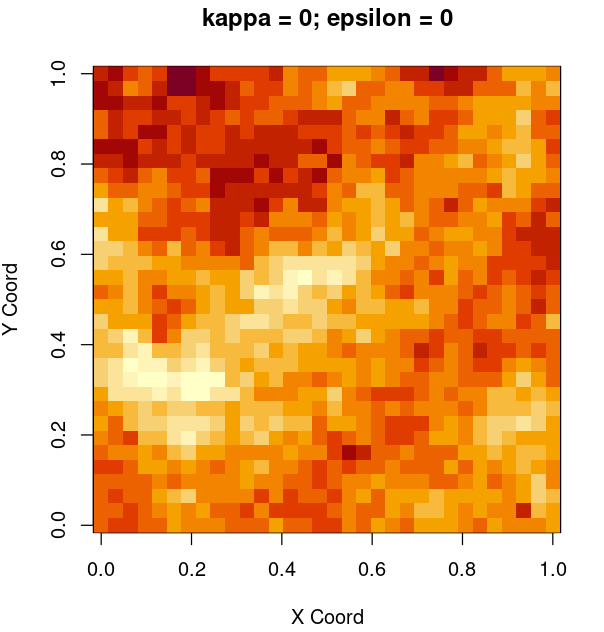
\includegraphics[width=3.125in,height=\textheight]{img/grf.png}
\end{center}

Then six different contaminated scenarios are simulated based on the
combinations of \(epsilon = (0.05, 0.1, 0.2)\) and \(kappa = (5, 10)\),
to assess the impact of contamination on the variogram estimation under
different circumstances.

\begin{center}
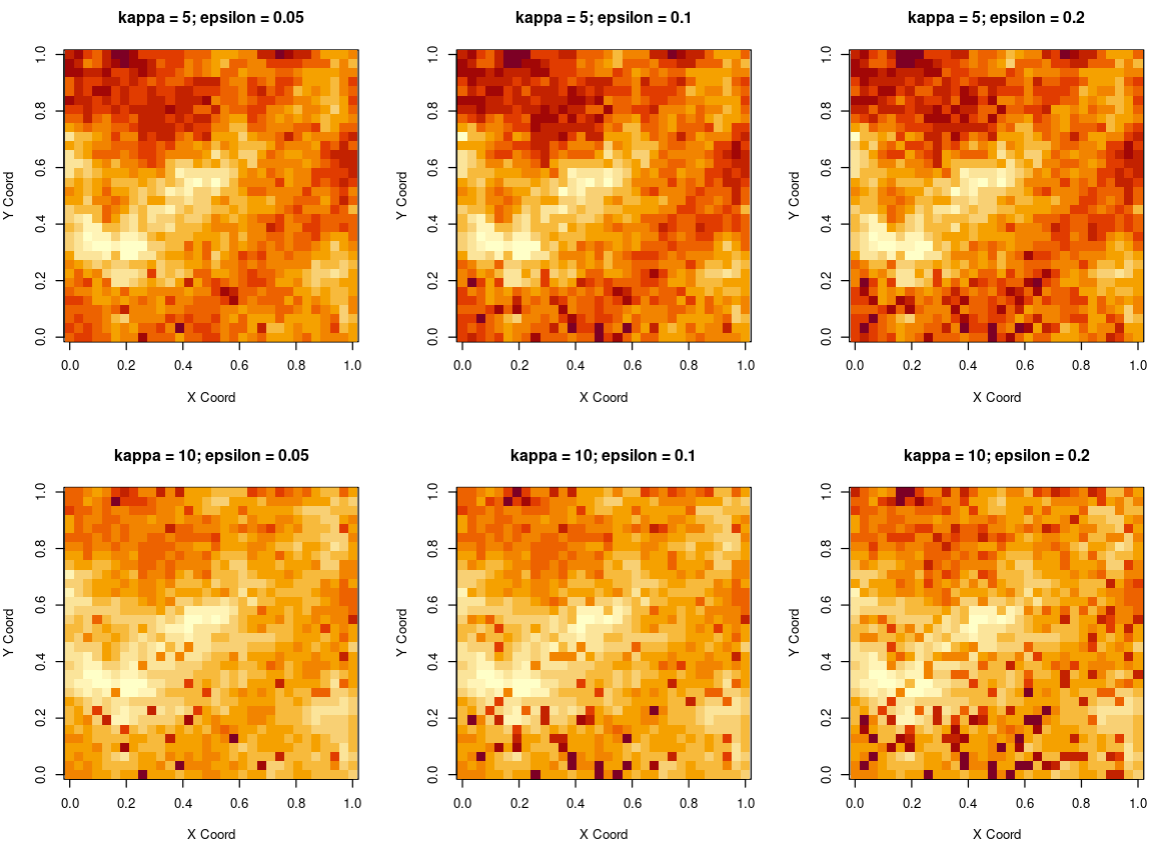
\includegraphics[width=5.20833in,height=\textheight]{img/cgrf.png}
\end{center}

Nugget and different levels of spatial correlation are not considered in
this simulation study but they can be easily added to the simulation
process.

\section{Results}\label{results}

The variogram estimation is performed using the classical (in black) and
the robust (in red) approaches. The two methods are compared on the
different simulated scenarios to assess their robustness to
contamination. Moreover, given that outliers are almost always
problematic for kriging, a variogram model is also estimated, using the
OLS estimator, to see how the outliers affect the model estimates. The
estimation process is performed using the functions variog and variofit
of the geoR package in R.

The base scenario, that is no contamination, shows that the two methods
provide almost identical results.

\begin{center}
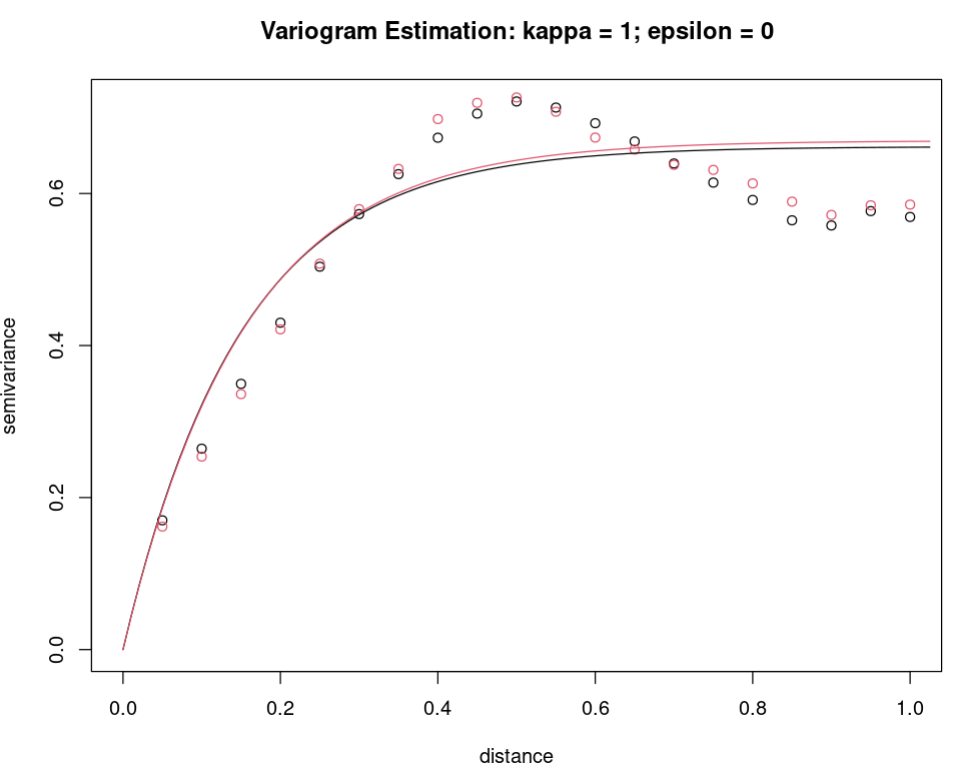
\includegraphics[width=5.20833in,height=\textheight]{img/variog_grf_ols.png}
\end{center}

In the presence of contamination, instead, the two methods provide
different results. If the results are analyzed in terms of the outliers'
scale (\(kappa\)), it is possible to observe two different behaviours.
For small outliers' scale, that is \(kappa = 5\), the two methods
provide similar estimations independently of the number of outliers
(\(\epsilon\)). However, for large outliers' scale, that is
\(kappa = 10\), the estimates are more different the higher the number
of outliers.

\begin{center}
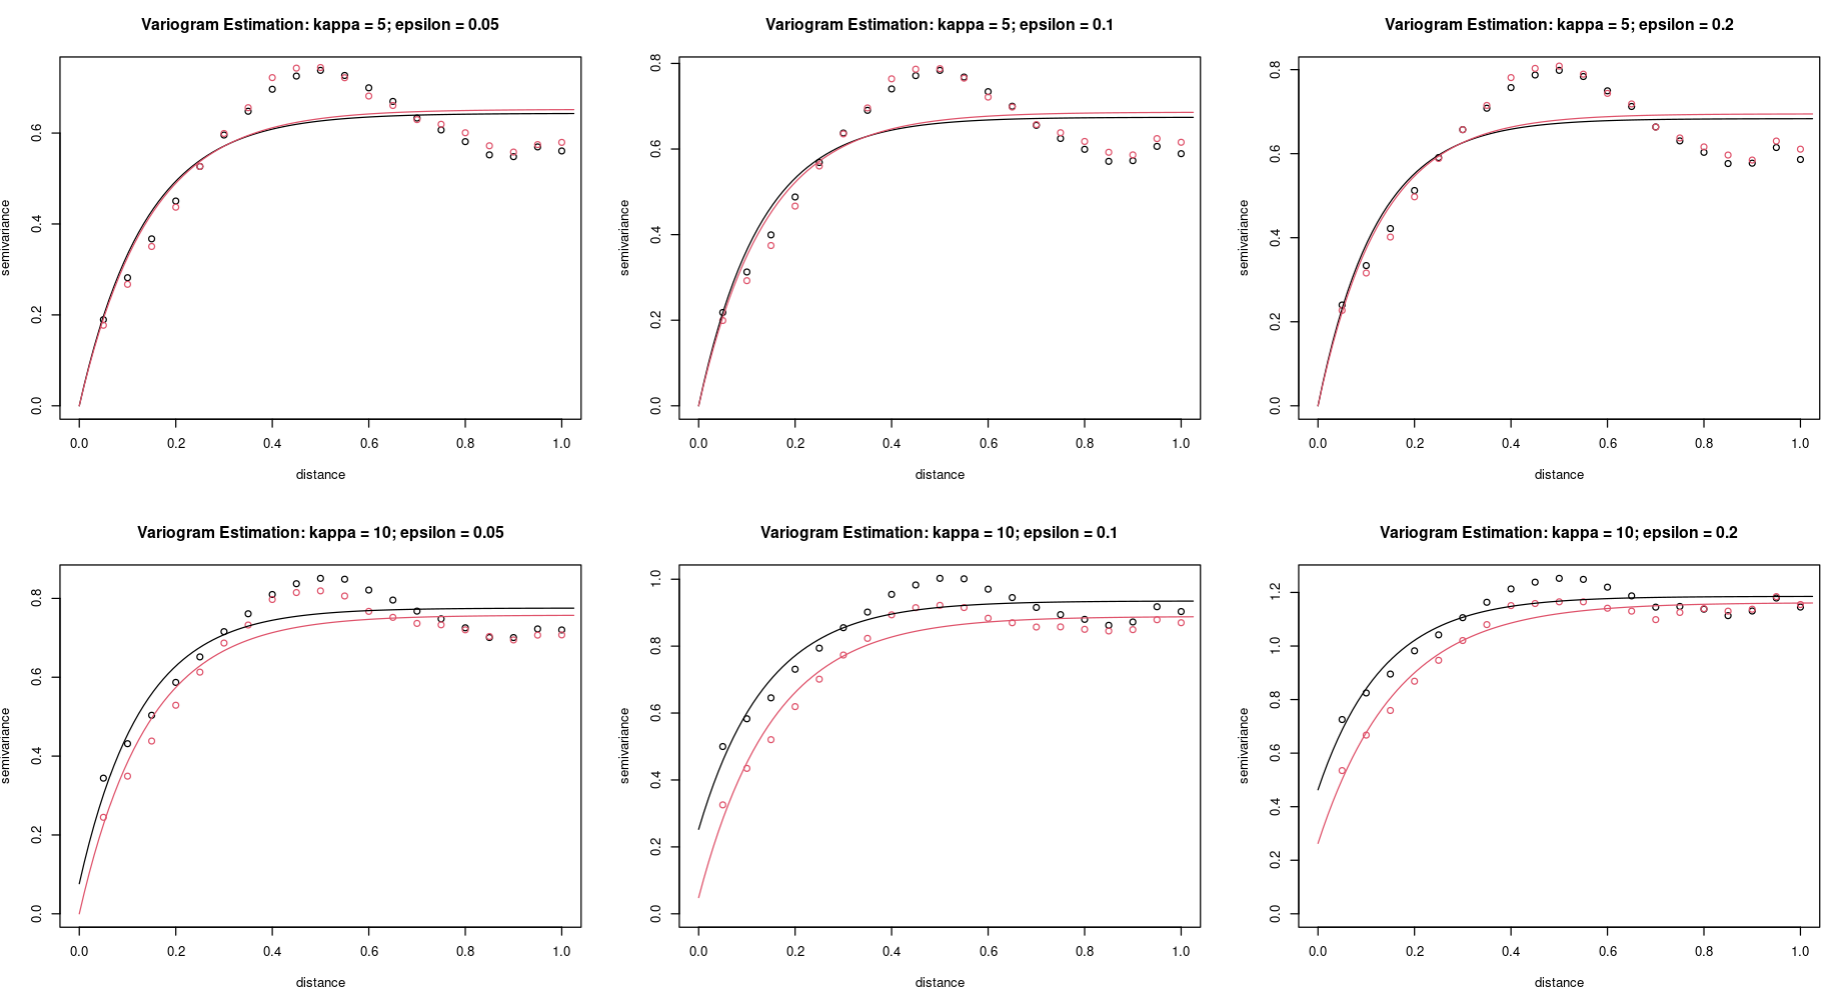
\includegraphics[width=6.25in,height=\textheight]{img/variog_cgrf_ols.png}
\end{center}

As expected, from theoretical considerations, the robust variogram
estimates are generally smaller than the classical ones. Indeed, the
classical approach is heavily influenced primarily by the scale of the
outliers, while the robust approach is less sensitive to the
contamination. Moreover, the scale of the contamination also strongly
affects the estimation of the nugget (which should be always 0), but the
robust approach is much less sensitive to this issue.

\begin{center}
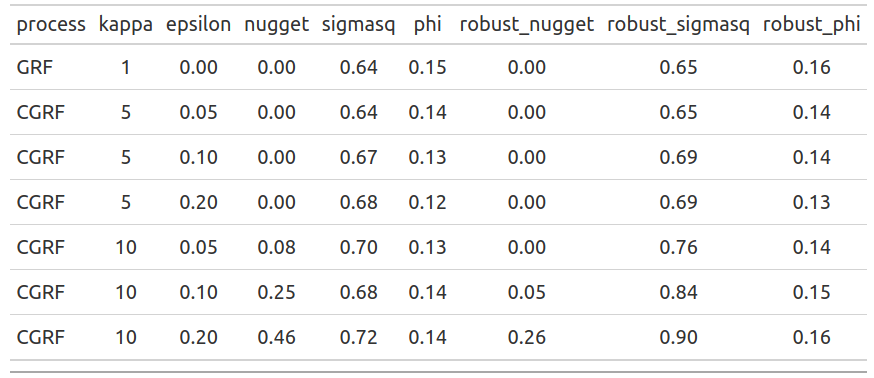
\includegraphics[width=6.25in,height=\textheight]{img/variog_est_ols.png}
\end{center}

\section{Conclusion}\label{conclusion}

The theoretical considerations suggest that the robust variogram is less
sensitive to the presence of outliers. For this reason it should be
preferred when the data are contaminated. The simulation study confirms
this results and shows that the robust variogram yields stable estimates
when the scale of the contamination increases. However, if the scale of
the contamination is small, then the two methods provide similar
results.


  \bibliography{bibliography.bib}


\end{document}
